\documentclass[conference]{IEEEtran}
\IEEEoverridecommandlockouts
% The preceding line is only needed to identify funding in the first footnote. If that is unneeded, please comment it out.
\usepackage{cite}
\usepackage{mathtools}
\usepackage{amsmath,amssymb,amsfonts}
\usepackage{algorithmic}
\usepackage{graphicx}
\usepackage{tikz}
\usepackage[mode=buildnew]{standalone}
\usepackage{subcaption} 
\usepackage{textcomp}
\usepackage{xcolor}
\def\BibTeX{{\rm B\kern-.05em{\sc i\kern-.025em b}\kern-.08em
    T\kern-.1667em\lower.7ex\hbox{E}\kern-.125emX}}
\begin{document}

\title{Decoding P300 Waveform plots based on Convolutional Neural Networks}


\author{\IEEEauthorblockN{1\textsuperscript{st} Brian Ezequiel Ail}
\IEEEauthorblockA{\textit{Computer Engineering Department} \\
\textit{Instituto Tecnológico de Buenos Aires}\\
Buenos Aires, Argentina \\
bail@itba.edu.ar}
\and
\IEEEauthorblockN{2\textsuperscript{nd} Rodrigo Ramele}
\IEEEauthorblockA{\textit{Computer Engineering Department} \\
\textit{Instituto Tecnológico de Buenos Aires}\\
Buenos Aires, Argentina \\
https://orcid.org/0000-0001-8155-0124}
\and
\IEEEauthorblockN{3\textsuperscript{rd} Juan Miguel Santos}
\IEEEauthorblockA{\textit{Computer Engineering Department} \\
\textit{Instituto Tecnológico de Buenos Aires}\\
Buenos Aires, Argentina \\
jsantos@itba.edu.ar}
%\and
%\IEEEauthorblockN{4\textsuperscript{th} Given Name Surname}
%\IEEEauthorblockA{\textit{dept. name of organization (of Aff.)} \\
%\textit{name of organization (of Aff.)}\\
%City, Country \\
%email address or ORCID}
%\and
%\IEEEauthorblockN{5\textsuperscript{th} Given Name Surname}
%\IEEEauthorblockA{\textit{dept. name of organization (of Aff.)} \\
%\textit{name of organization (of Aff.)}\\
%City, Country \\
%email address or ORCID}
%\and
%\IEEEauthorblockN{6\textsuperscript{th} Given Name Surname}
%\IEEEauthorblockA{\textit{dept. name of organization (of Aff.)} \\
%\textit{name of organization (of Aff.)}\\
%City, Country \\
%email address or ORCID}
}

\maketitle

\begin{abstract}
The use of Brain-Computer Interfaces can provide substantial improvements to the quality of life of patients with diseases such as severe Amyotrophic Lateral Sclerosis that could potentially derive in Locked-In syndrome, by creating new avenues in which these people can communicate and interact with the outside world. The P300 speller is an interface which provide the patients the ability to spell letters and eventually words, so that they can speak while unable to use their mouth. The P300 speller works by reading signals from the brain using an Electroencephalogram. Traditionally, these signals were plotted and interpreted by specialized technicians or neurologists, but the development of Machine learning algorithms for classification allow the computers to perform this analysis and detect the P300 signals, which is an Event Related Potential triggered when certain stimuli such as a bright light is triggered on a place that the patient is focused on. In this thesis we used a Convolutional Neural Network to train multi-channel EEG readings, and attempted to detect P300 signals from a P300 speller. The results are corroborated against a public ALS dataset.
\end{abstract}

\begin{IEEEkeywords}
component, formatting, style, styling, insert
\end{IEEEkeywords}

\section{Introduction}
\label{intro}

The understanding of the human brain has been one of the most exciting fields in recent history. The term psychokinesis and telekinesis has been around in science fiction for more than a century, from Luke Skywalker recalling his lightsaber using the Force, to Magneto  or Jean Grey of the X-Men. And what is telekinesis if not the movement of a physical object through signals emanating from the human brain?\cite{bcianiversary:10.1080/00051144.2019.1570644} The technology is not quite there at the moment, but it does not seem too far fetched to imagine right now, and not at all in the realm of science fiction. Controlling a prosthetic limb with the mind, or a monkey playing Pong\cite{neuralinkpong} with just his brain, are things that would have been unimaginable only a few years ago, but  cutting edge companies such as Neuralink are already working on invasive "high-bandwidth brain-machine interface system" \cite{info:neuralink/10.2196/16194}, which can make this kind of things a reality.

In terms of potential medical applications, patients with severe cases of Amyotrophic lateral sclerosis (ALS) can get into a 'Locked-in' state, in which they are unable to move any of their muscles to communicate. Creating a Brain-Computer interface can allow them to connect with the outside world  and substantially improve their quality of life\cite{GUY20185}.


This work proceeds as follows.  Section \ref{cite:background} introduces several implementations of affordable robotic architectures and cognitive solutions.  In the following section preliminaries definitions are exposed and the theoretical background is exposed.  The Materials and Methods section describes the hardware components and the cognitive architecture of this robotic platform, aimed to fulfill the requirements established in the previous section.  Benchmarks descriptios are exposed in the following section.  Results are expounded in the the following section and finally discussion and summaries are presented in the last section.

In the following sections we will take a look at how this classification can be performed using different algorithms such as Neural Networks, Support Vector Machines, or Scale Invariant Feature Transform, as well as the current state of the art  involving the use of such methods in recent years. Then we will discuss about our proposal for classification, which involves plotting the signals, and training a Convolutional Neural Network to identify the images, and finally compare these results to other studies performed using a common dataset of ALS patients.

Interpretable results or actionable analytics.

\subsection{Background}
\label{background}


As mentioned in section 1, the advance of hardware technologies, as well as the cheap accessibility of portable EEGs have significantly advanced the study of EEG signals using DNN. According to a 10 year study of Deep Learning in EEG\cite{dnn10years}, the amount of published papers that matched the searching criterion n [”Deep Learning” AND ”EEG” AND ”Classification” OR ”Recognition” OR ”Identification”] after manually curating the list, 213 papers had been published by march 2020. Out of these the vast majority of them were published from 2019 to 2020, and the trend is increasing rapidly. This papers include all range of studies of EEG, varying from Brain-Computer Interfaces to other applications such as Disease Detection, Sleep stage classification and Emotion recognition. 

When discussing applications of Deep Networks in BCI, they were a little hesitant, as Convolutional Networks are often used for computer vision or speech recognition, and did not match the requirements needed to analyze EEG signals. However they found many papers of successful applications of Convolutional Networks such as the work of Li et al.\cite{LI8709723}, which uses 3 different blocks of convolutional networks to decode motor imagery, which if successful would allow patients with loss of motor function to recover this lost mobility by the use of external devices. Liu et al. \cite{LIU2018288} used Batch Normalization to speed up the training and alleviate the overfitting. There are many other papers describing not only Deep Architectures for Brain Computer interfaces, but also for disease detection, mainly focusing on Epilepsy (with almost  50\% of the published papers) and Depression in second place with about 10\%.

Another review by Roy et al.\cite{RoyReview} specifically about using Deep Learning on EEG signals review a total of 156 papers. First of all, there is a very similar graph showing an increasing trend in the amount of published papers over the years, rising from less than 10 in 2014 to over 50 in 2018.


It also goes over most of the common problems, which we have also run into in this work. First of all regarding data imbalance, most papers with imbalanced data, such as epileptic seizure detection, or sleep stage transitions, used some form of class balancing, either by subsampling the majority class or by resampling the minority class on training.

For the DL architecture, the majority of the works used convolutional neural networks, with an overwhelming 41\%, while other architecture types such as autoencoders (AE) or recurrent neural networks (RNN) are under 14\%.

Regarding the amount of layers used, most architectures used from 2 to 7 layers, with  few examples over 7 layers,

Regarding regularization, 76 papers used some form of regularization, such as L1 or L2, dropout, or early stopping. While the other 80 do not mention regularization.

Finally, most papers (30\%) used the Adam method for optimization, while 17\% used Stochastic Gradient Descent, and 6\% used different optimizers.

This review gives us two big takeaways, first of all, it validates most of the choices used in the architecture proposed in our research. 
Another takeaway from both reviews, is that while Deep Learning seems like a big promise for the field of EEG, the field is still in it's early steps, the Deep Networks do not perform nowhere as good on EEG signals as they perform on other applications such as computer vision  or speech recognition. So it is still too early to say if Deep networks can perform as good as other learning algorithms, but if they can reach the same accuracy as they do on other applications, it can be a practical tool for EEG analysis.



\section{Materials and Methods}


\subsection{Software and Hardware}
The code ran on a HP Pavillion laptop with a Intel I7 @2.8GHz processor. The available RAM was 16Gb, although the software could run on much less RAM. A GPU was available, but the software did not run on a GPU.

The software for the signal segmentation, processing, and Signal drugging was written in python, using a modified version of the EEGWave repository from codeocean \cite{Ramele2018EEGWA}. It uses the MNE library for segmenting the data and some operations with numpy for signal processing.
The signal plotting is written in C++ using OpenCV, And the NN was run using Tensorflow's API for C++, based on Benny Friedman's article \cite{BennyCNN}. The full code is public and can be found at https://github.com/shipupi/BciSift/.


\subsection{P300 Experiment}
\subsubsection{Experiment Description}
The experiment was performed by Riccio et al., 2013\cite{riccio2013}. where a group of eight individuals with confirmed ALS disease were tasked to spell 7 5-letter words (35 total letters) with a P300 speller.

The first three words were used for calibration/training, while the remaining four were used for testing with visual feedback.

Each time a letter was attempted to be spelled is called a Trial. Each trial contained 10 flashes in each of the 6 rows, and 10 flashes in each of the 6 columns. The flashes lasted a total of 0.125 seconds each, followed by an inter-flashing pause of the same duration. After each 120 flashes, an inter-trial pause was performed before moving to the next letter.

The experiment was performed with an 8 channel EEG, with electrodes placed at the Fz, Cz, Pz, Oz, P3, P4, PO7, and PO8 channels according to the 10/20 international system. The software used for the flashing was the BCI2000 (open source) \cite{schalk2004}

The subjects were instructed to perform a copy-spelling task, which means that they have to spell a predetermined set of words that was instructed beforehand.


\begin{figure}[htbp]
\centerline{\includegraphics[width=8cm, keepaspectratio]{images/experiment.png}}
\caption[Experimental protocol visualization]{For each of the 35 letters, each row and column is highlighted 10 times, to allow for signal averaging. In each of these stimulus, if the column or row contains the target letter, we consider it a 'hit', while the columns and rows without the target letter are considered misses or 'nohits'. Since our EEG reads a total of 8 channels, the amount of total segments is calculated as 12 rows/columns x 10 repetitions x 8 channels  giving a total of 960 segments per letter. Since only a row and a column contain a hit while the others contain misses, we have 160 segments with hits and 800 segments with nohits.}
\label{fig:datastructure}
\end{figure}


\subsubsection{Dataset Structure}

After processing and segmenting the raw data. We can calculate the amount of segments generated by a single letter as follows:

\begin{equation}
N_l = (n_r + n_c)rc
\end{equation}
Where $n_r$ and $n_c$ are the number of rows and columns in the P300 matrix, $c$ is the amount of channels i.e. the amount of electrodes on the EEG, and $r$ is the amount of repetitions done per letter.

In the ALS experiment, the data was recorded using an 8-channel EEG, and 10 repetitions were performed per letter. The P300 matrix contained 6 rows and 6 columns, this results in a total of 960 segments per single letter. There is a single row and a single column with the P300 signal, and 5 rows and 5 columns without it. This results in each letter being segmented into 160 hits, and 800 nohits.

The experiment was performed using 7 5-letter words, resulting in 35 letters, and a total of 33600 segments. Out of these, 15 letters were used for the training of the networks, and the remaining 20 were used to test the accuracy.


Explain the three networks.

\subsection{VGG16 Neural Network}

\begin{figure*}[!t]
\includestandalone[width=18cm, keepaspectratio]{images/nnv1}
\caption[VGG16 Neural Network]{First version of the NN, a set of 5 convolutional layers is followed by 4 fully connected layer, and finally activated using a sigmoid function}
\label{fig:nnv1}
\end{figure*}


The first version of the neural network was based on VGG16, a deep network which was used to win the ImageNet Large Scale Visual Recognition Challenge (ILSVR) competition in 2014\cite{ilsvr2014}. It uses a 3x3 filter with a stride of 1 and uses padding to keep the same spatial dimensions, followed by a MaxPool layer of 2x2 size and stride 2, and follows this arrangement of convolution and maxpool layers all the way throughout the whole architecture, for 5 convolutional + maxpool sets. In the end, the VGG16 has 2 fully connected (regular neural network) layers, while we are using 4. In the end, the last layer is activated with a sigmoid function to make the binary classification. 
The advantage of the VGG16 approach, is that it reduces the amount of hyperparameters that must be tinkered with, as all the filters and strides are kept constant. 

Our network has 6 convolutional layers with a depth of 1, 32, 64, 128, 128 and 256. The stride in the maxpool reduces the spatial size in each iteration, leaving a spatial size of 150, 75, 38, 19, 10, 5 (the images are squared, so width and height are the same). 

After the convolutional layers, a dropout layer with a drop rate of 0.5, and a flatten layer to make the data ready for the dense layers. The 4 dense layers have a size of 6400, 1024, 512 and 256 units, with the last one having a sigmoid activation.

The learning algorithm was the stochastic gradient descent method called Adam\cite{adam2014}, and the loss function was the means squared difference. And it was done in batches of size 20. 

The learning rate used was $5\,10^{-4}$, which deviates from the recommended $3\, 10^{-3}$. This parameter was tinkered with for a bit, and was the suspect of the Network not convering at first, so decreasing the learning rate helped a bit.

Ultimately, the convergence issue was solved by balancing the dataset, first by prunning some of the misses in, and in later versions by duplicating the hits, as this latter method allowed the use of all the misses.

After training with the first 15 letters, the network was used to predict the remaining 20 letters, and the performance of the network was calculated by finding the row and column with the highest predicted change of containing the P300 signal and comparing the predicted letter to the original expected letter from the experiment.

These predictions were done by training each of the EEG channels separately, and then finding the channel that best perform. As mentioned early, another prediction was used by making a non-weighted voting system by each of the channels, and selecting the row and column with the most votes.

Since we are running what is considered a 'BCI Simulation'. The training was performed only once, instead of multiple runs doing cross validation or calculating mean and standard deviation in the accuracies. This is because we want to simulate a real use case of a patient actually using our interface.

\subsection{Small VGG16}
\begin{figure*}[h]
\centering
\includestandalone[width=18cm, keepaspectratio]{images/nnv2}
\caption[SVG16 Neural Network]{SV16 is similar to VGG16, but has two less convolutional layers and two less dense layers}
\label{fig:nnv2}
\end{figure*}

The second approach was the Small VGG16  (SV16). The first change was to reduce the network size, so 2 convolutional layers and 2 fully connected layers were removed. Leaving the convolutional layers depth at 1, 32, 64 and 128, with spatial sides of 150, 75, 38, and 19. The flatten and dropout layers are left untouched, and then finally 3 fully connected layers of sizes 46208, 512 and 256. The overall philosophy of the architecture was left untouched, i.e. the padding, filter size and stride.

Another addition in this version was early stopping at 7 epochs to help decrease overfitting. 

\subsection{Multichannel Small VGG16 (MSV16)}

\begin{figure*}[h]
\includestandalone[width=18cm, keepaspectratio]{images/nnv3}
\caption[MSV16 Neural Network]{MSV16 has the same architecture as the second one, but the input layer is modified for an 8-channel input}
\label{fig:nnv3}
\end{figure*}

With this multichannel network, instead of training all of the EEG channels separately, they were merged into a single 8-channel image on the preprocessing stage. And the network was trained with this image as input. This modified the input layer to have a depth of 8, but the subsequent layers were left intact. The best improvement was that it allowed for the combination of all the different EEG channels to work together, achieving a higher performance than each channel separately.

To make this change work however, extra changes had to be made to the network parameters. The batch size was reduced to 6, as having a greater batch size generated memory issues. The last change was reducing the learning rate to the recommended value of $3\cdot10^-3$.

\section{Results}
\label{sec:results}


\subsection{Validation on the Pseudoreal dataset}


\begin{table}[h]
\centering
\begin{tabular}{ |p{1cm}||p{1cm}|p{1cm}|p{1cm}|p{1cm}|p{1cm}| }
 \hline
 Subject & VGG16(\%) & SV16 (\%)  & MSV16(\%) & HIST(\%)\\
 \hline
 1 & 15 & 10 & 0 & 35\\
 2 & 70 & 50 & 75 & 85\\
 3 & 30 & 30 & 40 & 25\\
 4 & 30 & 40 & 30 & 55\\
 5 & 35 & 50 & 50 & 40\\
 6 & 45 & 40 & 50 & 60\\
 7 & 70 & 65 & 80 & 80\\
 8 & 90 & 95 & 100 & 95\\
 \hline
\end{tabular}
\caption[MSV16 accuracy comparison]{Character recognition rates for VGG16, SV16, MSV16 and HIST}
\label{tab:resultsv1v2v3}
\end{table}
\begin{figure}[h]
  \centering
  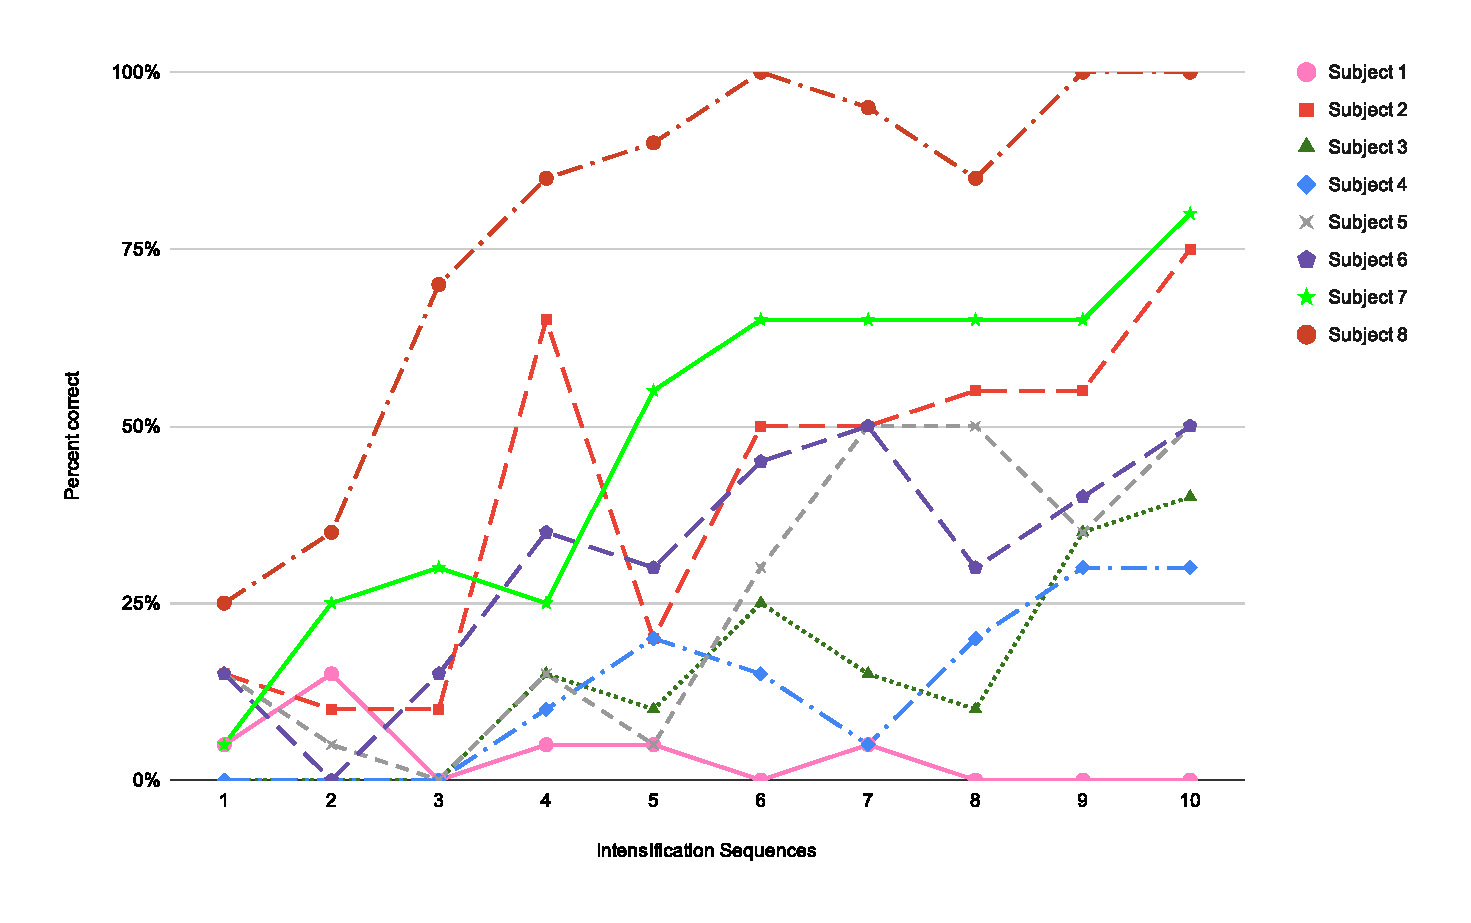
\includegraphics[width=\linewidth]{images/v3intensification.eps}
  \caption[MSV16 Letter accuracy]{Letter accuracy for MSV16 shows a significant improvement over SV16}
  \label{image:v3intensification}
\end{figure}
The third and final version of the network included both the improvements made in SV16, as well as the addition of multi-channel classification, and a smaller batch size. The results can be seen in \ref{tab:resultsv1v2v3}. This last version showed an accuracy increase in 6 out of 8 channels over the other two versions. It surpasses HIST in 3 out of 8 subjects, and performs equally on 1. 
It does however seem to underperform on subject 1 and 4 compared to earlier versions and HIST. But it also reaches a 100\% accuracy on subject 8, which none of the other methods had managed to achieve.
Also, by looking at the accuracy per intensification level, subject 8 achieved over 90\% accuracy in only 5 repetitions, meaning that a robust speller could be established with a much faster transmission rate. 

The learning curve for subject 5 at an intensification level of 4 can be seen in \ref{image:v3curve}. If compared to the same curve in the first network \ref{image:v1curve}, the accuracy for the validation set is much higher, while the accuracy of the training set remains at or close to 100\%. This suggests that there is still some overfitting left to solve, which would indicate that this method still has potential to find even higher success.


\begin{figure}[h]
  \centering
  \includegraphics[width=\linewidth]{images/v3curve.eps}
  \caption[MSV16 Learning curve]{Learning curve of subject 5, with an intensification level of 4 using multichannel training}
  \label{image:v3curve}
\end{figure}




\section{Discussion}


\subsubsection{Results validation}
While there is no fail-proof way of assuring that the code is running bug-free, certain automatic and manual fail safes have been included to make the assertion that the results are valid.

When generating the training data, only the 15 letters are plotted. The remaining 20 letters are completely ignored, there is no possibility that the training used any of the testing set. 

Generating the testing set follows a similar process, as the plotting is only performed on the last 20 letters, and the plots for the first 15 letters are deleted from the hard drive.

When averaging the signals, the standard deviation of the resulting signals is calculated, and it is asserted that the new standard deviation is indeed lower than the original one.

To corroborate that the results were not random, a training of the dataset was performed by randomizing the labels, the expected outcome of this is that the predictions for the letters are completely random. We can see this in figure \ref{image:randomlabels}, the accuracy of the training done with random labels on subject 8 with MSV16 is oscillating around the random threshold, which is 1/36, or 3\%, while the same training without randomizing the labels on the training goes back up to the regular accuracies. This shows that there is indeed a generalization being performed by the network, and the results are not 'by chance'.

\begin{figure}[htb]
  \centering
  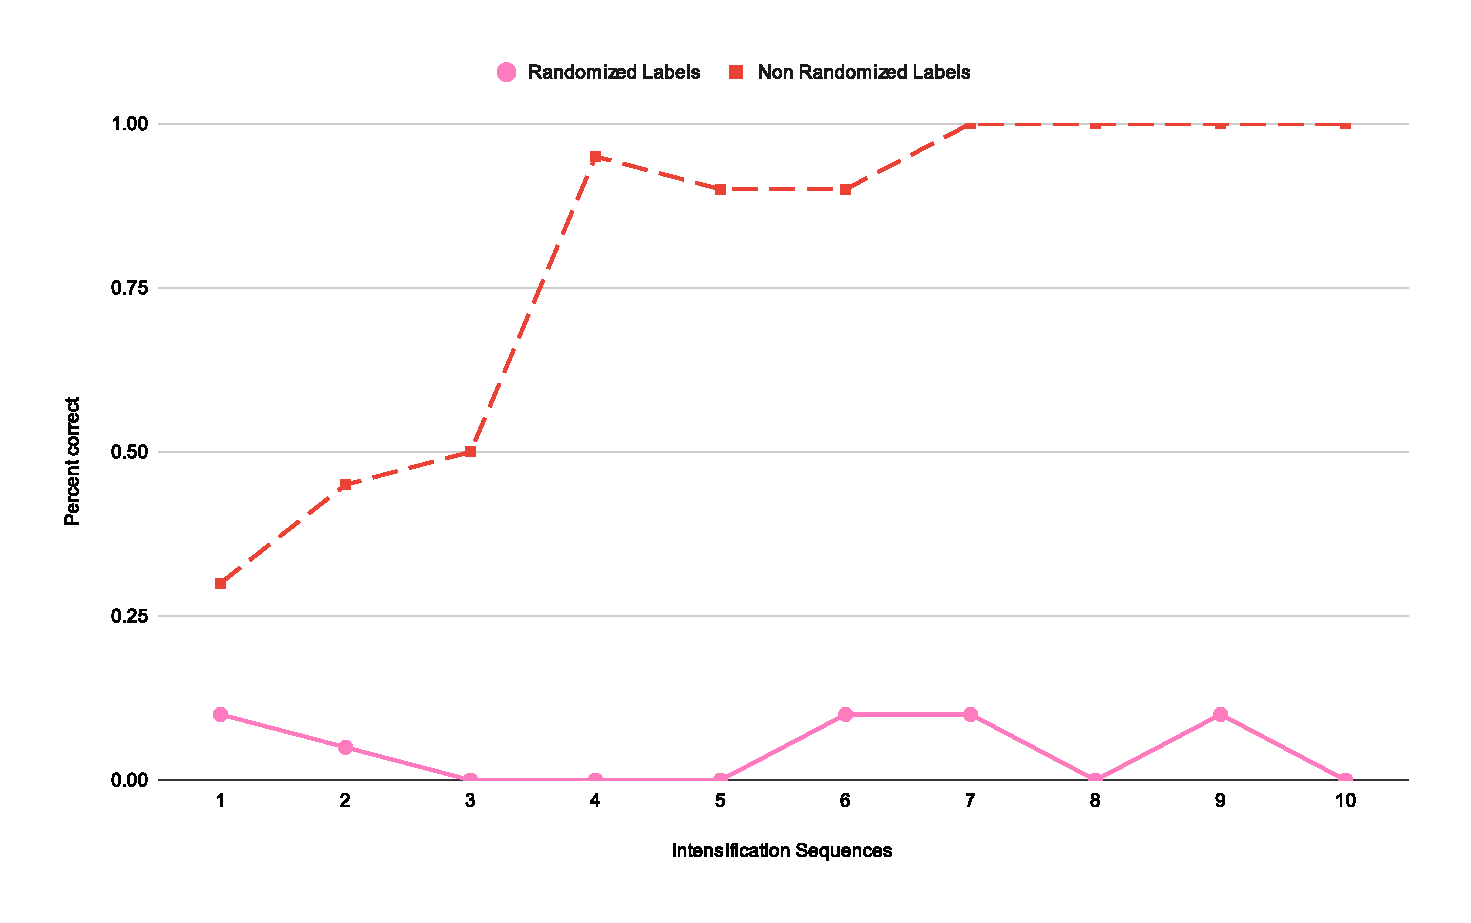
\includegraphics[width=\linewidth]{images/randomlabels.eps}
  \caption[Random Labels Accuracy]{Accuracy of MSV16 on subject 8, the red line shows a normal prediction using regular labels on the training set, while the pink line shows the predictions of the NN by training it with randomized labels on the training set. We can see that the accuracy on the pink line hovers around the \emph{random} range(3\%)}
  \label{image:randomlabels}
\end{figure}

The most telling assurance however, is that the results are consistent with previous works on the same dataset such as \cite{ramele2019histogram}. The accuracy curves for the different subjects, while not exactly identical, follow similar patterns, such as the subject 8 performing very well, while subject 1 performs badly. And the accuracy is consistently increasing along with the intensification level.


\subsubsection{Drugged signals}
When we generate a drugged dataset with a boost level of 0, we get a purely basal EEG signal, when encountering this dataset, the network should learn and converge, but the accuracy on the testing set should perform very bad, close to random levels, as there is no pattern to generalize. This can be seen on figure \ref{image:boosted0curve}, while the training accuracy (red line) increases, the testing accuracy (yellow line) is stuck around 50\%, which means that the prediction is completely random.

When moving on to a boost level of 1, the signal is very similar to the subject 8 of the ALS dataset, this gave us a preview of how the network behaved and learned on a real dataset. On figure \ref{image:boostintensification} the boosted 1 curve (red line) performs pretty well, reaching almost 50\% accuracy when averaging 10 signals (note: the threshold for random letter accuracy is 1/36$\approx$3\%).

As the boost levels increased, the P300 became more dominant in the signal and the SNR decreased, making the images easier to classify, thus the expectation is that when the level of boost increases, the accuracy increases as well, which we can see on figure \ref{image:boosttransposed}.

\subsubsection{DL performance}

Regarding the VGG16 architecture, we  can see in figure \ref{image:v1curve} that the main issue is overfitting. The training sets are being learned perfectly, reaching a 100\% accuracy, but the accuracy on the validation set does not increase, and oscillates around 60\%, while this is a bit better than random level values, it still needs improvement. Figure \ref{image:v1curve} is just one of the many learning curves drawn for this version, but it showcases the overfitting problem.

The SV16 version attempted to address this issue by adding early stopping and reducing the amount of layers, as shown on table \ref{tab:resultsv1v2}, the improvement on letter accuracy from these changes seems small, as the results are barely better, but it should be taken into account that the results for VGG16 are taken with the best performing channel, while the results for SV16 are only taken from training on the PO8 channel, so even a similar result is a good indicator.

The biggest breakthrough of this work however is the MSV16 version, the inclusion of all the EEG channels into a single image, generated substantial improvements compared to both previous versions, and it even surpassed other proven methods such as SVM and HIST on some of the subjects, proving that using DL methods for this task is a very viable option. For some reason however, it performed very poorly on subject 1, although most of the DL methods did, while the HIST method can get a 35\% accuracy on it.


\begin{figure}[h]
    %IMAGEN 1
    \begin{subfigure}[t]{0.5\textwidth}
    \centering\captionsetup{width=.8\linewidth}
    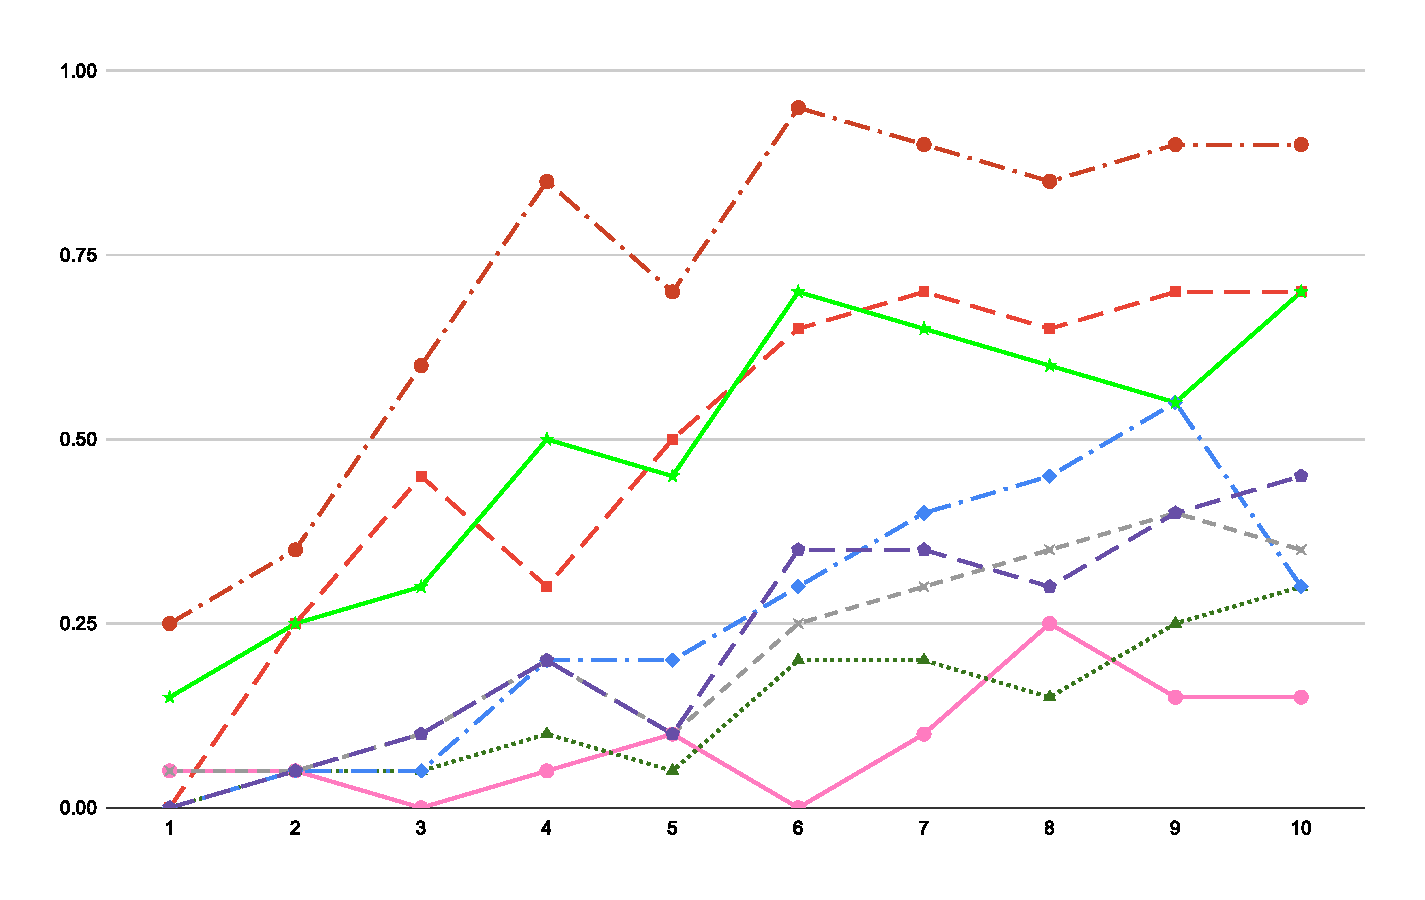
\includegraphics[width=1\linewidth, keepaspectratio]{images/v1intensificationnolabel.eps}
    \caption{Letter accuracy for VGG16 \label{image:v1intensification2}}
    \end{subfigure}
    %IMAGEN 2
    \begin{subfigure}[t]{0.5\textwidth}
    \centering\captionsetup{width=.8\linewidth}
    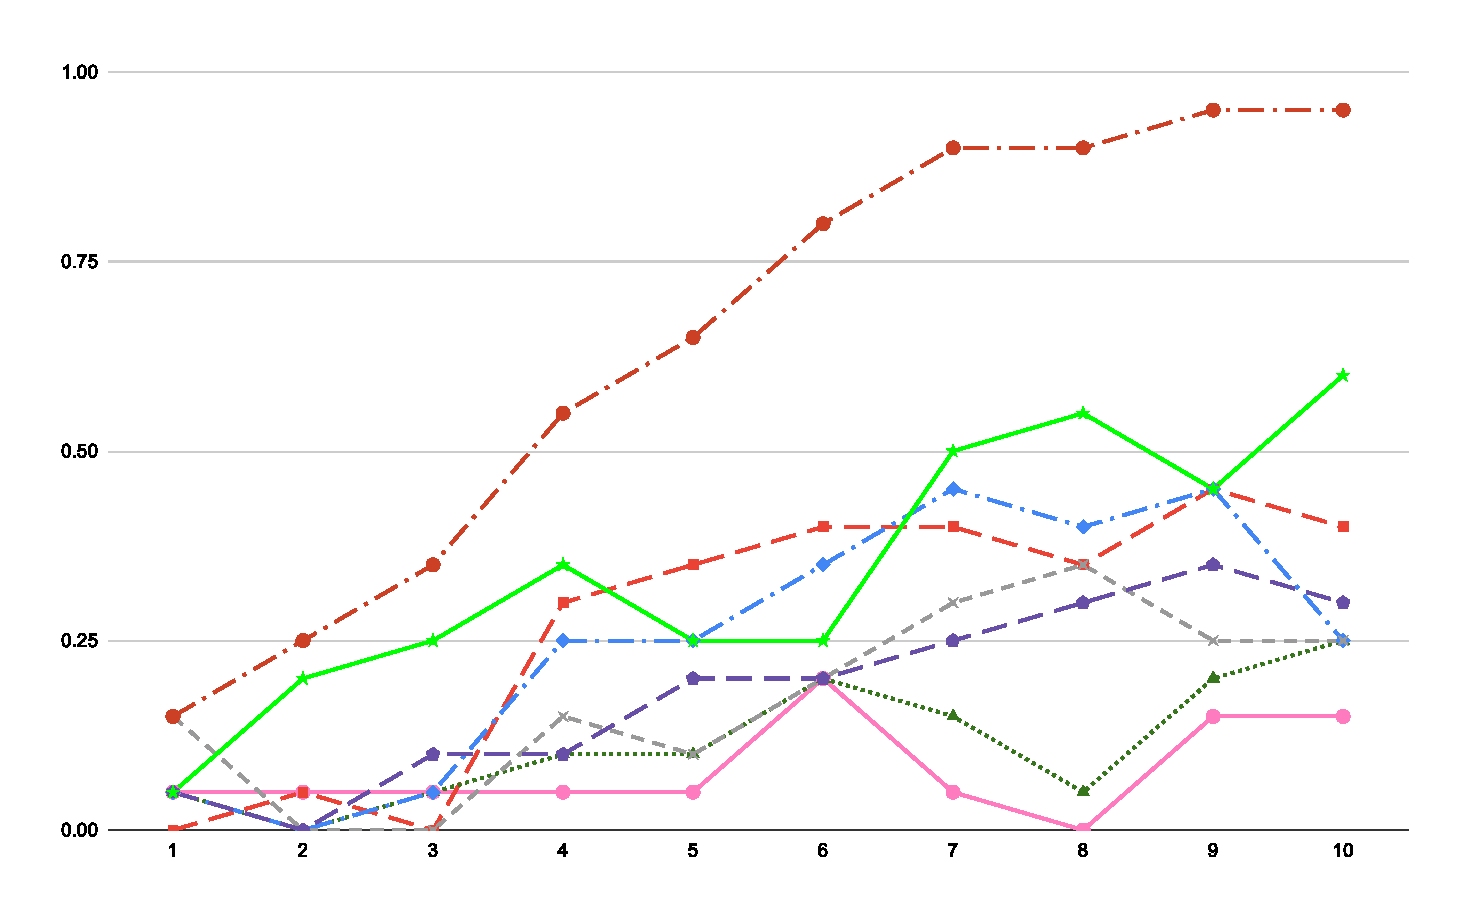
\includegraphics[width=1\linewidth, keepaspectratio]{images/v2intensificationnolabel.eps}
    \caption{Letter accuracy for SV16 \label{image:v2intensification2}}
    \end{subfigure}
    %IMAGEN 3
    \begin{subfigure}[t]{0.5\textwidth}
    \centering\captionsetup{width=.8\linewidth}
    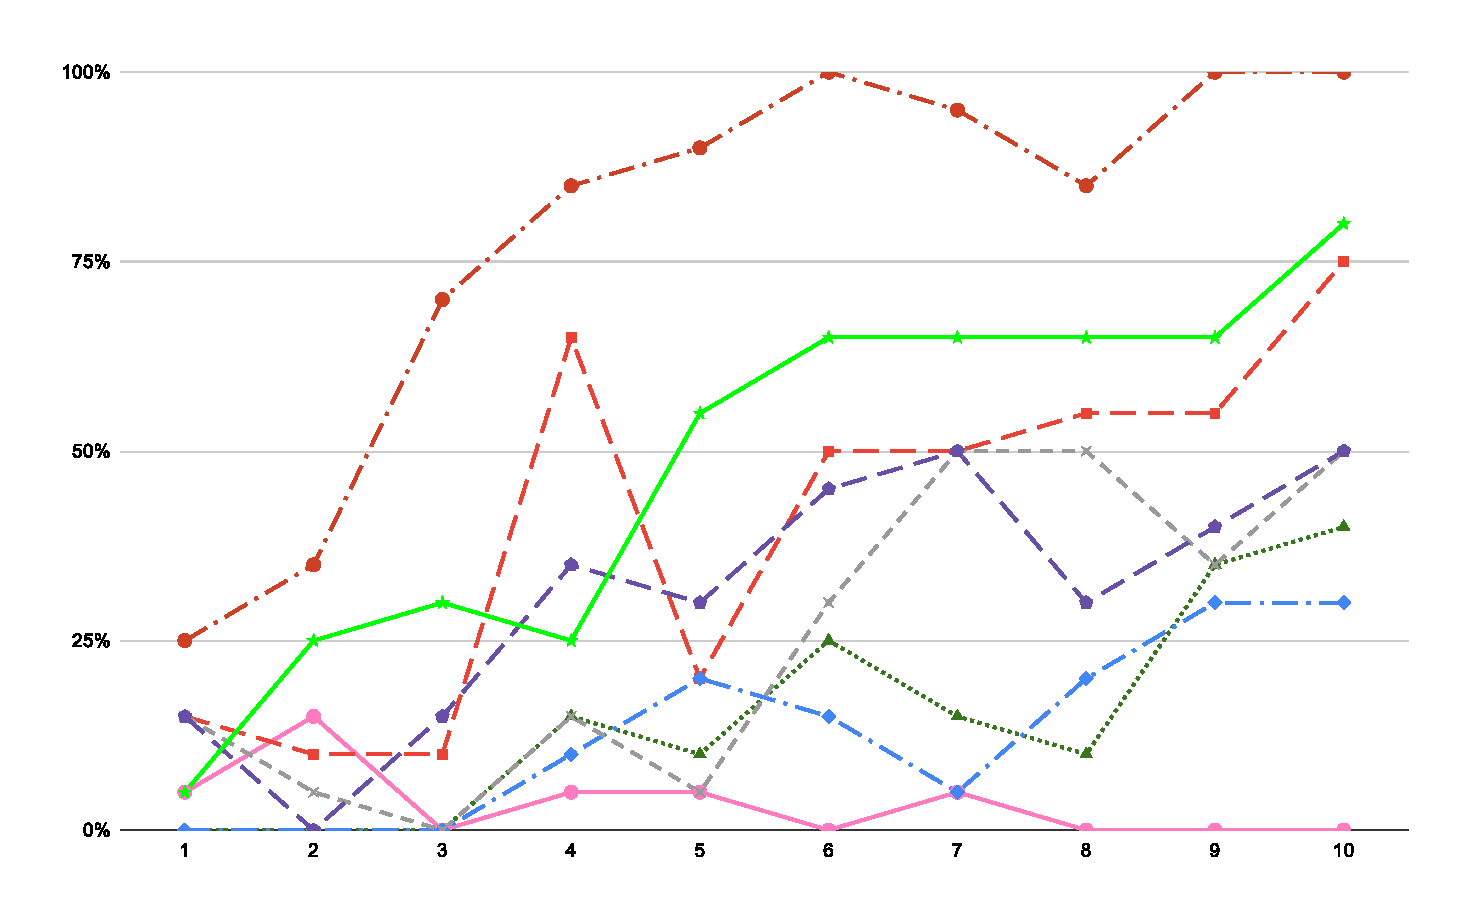
\includegraphics[width=1\linewidth, keepaspectratio]{images/v3intensificationnolabel.eps}
    \caption{Letter accuracy for MSV16 \label{image:v3intensification2}}
    \end{subfigure}
     %IMAGEN 4
    \begin{subfigure}[t]{0.5\textwidth}
    \centering\captionsetup{width=.8\linewidth}
    \includegraphics[width=0.7\linewidth, keepaspectratio]{images/histintensification.jpg}
    \caption{Letter accuracy for HIST method \cite{ramele2019histogram} \label{image:histintensification}}
    \end{subfigure}
    
    %CAPTION FINAL
    \caption[Letter accuracy for all architectures ]{Side by side comparison of all the architectures, and finally a comparison to the HIST method, original figures can be found on section \ref{sect:results}}\label{image:allversionsiaccuracy}
\end{figure}



%\section{Ease of Use}
%
%\subsection{Maintaining the Integrity of the Specifications}
%
%The IEEEtran class file is used to format your paper and style the text. All margins, 
%column widths, line spaces, and text fonts are prescribed; please do not 
%alter them. You may note peculiarities. For example, the head margin
%measures proportionately more than is customary. This measurement 
%and others are deliberate, using specifications that anticipate your paper 
%as one part of the entire proceedings, and not as an independent document. 
%Please do not revise any of the current designations.
%
%\section{Prepare Your Paper Before Styling}
%Before you begin to format your paper, first write and save the content as a 
%separate text file. Complete all content and organizational editing before 
%formatting. Please note sections \ref{AA}--\ref{SCM} below for more information on 
%proofreading, spelling and grammar.
%
%Keep your text and graphic files separate until after the text has been 
%formatted and styled. Do not number text heads---{\LaTeX} will do that 
%for you.
%
%\subsection{Abbreviations and Acronyms}\label{AA}
%Define abbreviations and acronyms the first time they are used in the text, 
%even after they have been defined in the abstract. Abbreviations such as 
%IEEE, SI, MKS, CGS, ac, dc, and rms do not have to be defined. Do not use 
%abbreviations in the title or heads unless they are unavoidable.
%
%\subsection{Units}
%\begin{itemize}
%\item Use either SI (MKS) or CGS as primary units. (SI units are encouraged.) English units may be used as secondary units (in parentheses). An exception would be the use of English units as identifiers in trade, such as ``3.5-inch disk drive''.
%\item Avoid combining SI and CGS units, such as current in amperes and magnetic field in oersteds. This often leads to confusion because equations do not balance dimensionally. If you must use mixed units, clearly state the units for each quantity that you use in an equation.
%\item Do not mix complete spellings and abbreviations of units: ``Wb/m\textsuperscript{2}'' or ``webers per square meter'', not ``webers/m\textsuperscript{2}''. Spell out units when they appear in text: ``. . . a few henries'', not ``. . . a few H''.
%\item Use a zero before decimal points: ``0.25'', not ``.25''. Use ``cm\textsuperscript{3}'', not ``cc''.)
%\end{itemize}
%
%\subsection{Equations}
%Number equations consecutively. To make your 
%equations more compact, you may use the solidus (~/~), the exp function, or 
%appropriate exponents. Italicize Roman symbols for quantities and variables, 
%but not Greek symbols. Use a long dash rather than a hyphen for a minus 
%sign. Punctuate equations with commas or periods when they are part of a 
%sentence, as in:
%\begin{equation}
%a+b=\gamma\label{eq}
%\end{equation}
%
%Be sure that the 
%symbols in your equation have been defined before or immediately following 
%the equation. Use ``\eqref{eq}'', not ``Eq.~\eqref{eq}'' or ``equation \eqref{eq}'', except at 
%the beginning of a sentence: ``Equation \eqref{eq} is . . .''
%
%\subsection{\LaTeX-Specific Advice}
%
%Please use ``soft'' (e.g., \verb|\eqref{Eq}|) cross references instead
%of ``hard'' references (e.g., \verb|(1)|). That will make it possible
%to combine sections, add equations, or change the order of figures or
%citations without having to go through the file line by line.
%
%Please don't use the \verb|{eqnarray}| equation environment. Use
%\verb|{align}| or \verb|{IEEEeqnarray}| instead. The \verb|{eqnarray}|
%environment leaves unsightly spaces around relation symbols.
%
%Please note that the \verb|{subequations}| environment in {\LaTeX}
%will increment the main equation counter even when there are no
%equation numbers displayed. If you forget that, you might write an
%article in which the equation numbers skip from (17) to (20), causing
%the copy editors to wonder if you've discovered a new method of
%counting.
%
%{\BibTeX} does not work by magic. It doesn't get the bibliographic
%data from thin air but from .bib files. If you use {\BibTeX} to produce a
%bibliography you must send the .bib files. 
%
%{\LaTeX} can't read your mind. If you assign the same label to a
%subsubsection and a table, you might find that Table I has been cross
%referenced as Table IV-B3. 
%
%{\LaTeX} does not have precognitive abilities. If you put a
%\verb|\label| command before the command that updates the counter it's
%supposed to be using, the label will pick up the last counter to be
%cross referenced instead. In particular, a \verb|\label| command
%should not go before the caption of a figure or a table.
%
%Do not use \verb|\nonumber| inside the \verb|{array}| environment. It
%will not stop equation numbers inside \verb|{array}| (there won't be
%any anyway) and it might stop a wanted equation number in the
%surrounding equation.
%
%\subsection{Some Common Mistakes}\label{SCM}
%\begin{itemize}
%\item The word ``data'' is plural, not singular.
%\item The subscript for the permeability of vacuum $\mu_{0}$, and other common scientific constants, is zero with subscript formatting, not a lowercase letter ``o''.
%\item In American English, commas, semicolons, periods, question and exclamation marks are located within quotation marks only when a complete thought or name is cited, such as a title or full quotation. When quotation marks are used, instead of a bold or italic typeface, to highlight a word or phrase, punctuation should appear outside of the quotation marks. A parenthetical phrase or statement at the end of a sentence is punctuated outside of the closing parenthesis (like this). (A parenthetical sentence is punctuated within the parentheses.)
%\item A graph within a graph is an ``inset'', not an ``insert''. The word alternatively is preferred to the word ``alternately'' (unless you really mean something that alternates).
%\item Do not use the word ``essentially'' to mean ``approximately'' or ``effectively''.
%\item In your paper title, if the words ``that uses'' can accurately replace the word ``using'', capitalize the ``u''; if not, keep using lower-cased.
%\item Be aware of the different meanings of the homophones ``affect'' and ``effect'', ``complement'' and ``compliment'', ``discreet'' and ``discrete'', ``principal'' and ``principle''.
%\item Do not confuse ``imply'' and ``infer''.
%\item The prefix ``non'' is not a word; it should be joined to the word it modifies, usually without a hyphen.
%\item There is no period after the ``et'' in the Latin abbreviation ``et al.''.
%\item The abbreviation ``i.e.'' means ``that is'', and the abbreviation ``e.g.'' means ``for example''.
%\end{itemize}
%An excellent style manual for science writers is \cite{b7}.
%
%\subsection{Authors and Affiliations}
%\textbf{The class file is designed for, but not limited to, six authors.} A 
%minimum of one author is required for all conference articles. Author names 
%should be listed starting from left to right and then moving down to the 
%next line. This is the author sequence that will be used in future citations 
%and by indexing services. Names should not be listed in columns nor group by 
%affiliation. Please keep your affiliations as succinct as possible (for 
%example, do not differentiate among departments of the same organization).
%
%\subsection{Identify the Headings}
%Headings, or heads, are organizational devices that guide the reader through 
%your paper. There are two types: component heads and text heads.
%
%Component heads identify the different components of your paper and are not 
%topically subordinate to each other. Examples include Acknowledgments and 
%References and, for these, the correct style to use is ``Heading 5''. Use 
%``figure caption'' for your Figure captions, and ``table head'' for your 
%table title. Run-in heads, such as ``Abstract'', will require you to apply a 
%style (in this case, italic) in addition to the style provided by the drop 
%down menu to differentiate the head from the text.
%
%Text heads organize the topics on a relational, hierarchical basis. For 
%example, the paper title is the primary text head because all subsequent 
%material relates and elaborates on this one topic. If there are two or more 
%sub-topics, the next level head (uppercase Roman numerals) should be used 
%and, conversely, if there are not at least two sub-topics, then no subheads 
%should be introduced.
%
%\subsection{Figures and Tables}
%\paragraph{Positioning Figures and Tables} Place figures and tables at the top and 
%bottom of columns. Avoid placing them in the middle of columns. Large 
%figures and tables may span across both columns. Figure captions should be 
%below the figures; table heads should appear above the tables. Insert 
%figures and tables after they are cited in the text. Use the abbreviation 
%``Fig.~\ref{fig}'', even at the beginning of a sentence.
%
%\begin{table}[htbp]
%\caption{Table Type Styles}
%\begin{center}
%\begin{tabular}{|c|c|c|c|}
%\hline
%\textbf{Table}&\multicolumn{3}{|c|}{\textbf{Table Column Head}} \\
%\cline{2-4} 
%\textbf{Head} & \textbf{\textit{Table column subhead}}& \textbf{\textit{Subhead}}& \textbf{\textit{Subhead}} \\
%\hline
%copy& More table copy$^{\mathrm{a}}$& &  \\
%\hline
%\multicolumn{4}{l}{$^{\mathrm{a}}$Sample of a Table footnote.}
%\end{tabular}
%\label{tab1}
%\end{center}
%\end{table}
%
%\begin{figure}[htbp]
%\centerline{\includegraphics{fig1.png}}
%\caption{Example of a figure caption.}
%\label{fig}
%\end{figure}
%
%Figure Labels: Use 8 point Times New Roman for Figure labels. Use words 
%rather than symbols or abbreviations when writing Figure axis labels to 
%avoid confusing the reader. As an example, write the quantity 
%``Magnetization'', or ``Magnetization, M'', not just ``M''. If including 
%units in the label, present them within parentheses. Do not label axes only 
%with units. In the example, write ``Magnetization (A/m)'' or ``Magnetization 
%\{A[m(1)]\}'', not just ``A/m''. Do not label axes with a ratio of 
%quantities and units. For example, write ``Temperature (K)'', not 
%``Temperature/K''.

\section*{Acknowledgment}

The preferred spelling of the word ``acknowledgment'' in America is without 
an ``e'' after the ``g''. Avoid the stilted expression ``one of us (R. B. 
G.) thanks $\ldots$''. Instead, try ``R. B. G. thanks$\ldots$''. Put sponsor 
acknowledgments in the unnumbered footnote on the first page.

\section*{References}

Please number citations consecutively within brackets \cite{b1}. The 
sentence punctuation follows the bracket \cite{b2}. Refer simply to the reference 
number, as in \cite{b3}---do not use ``Ref. \cite{b3}'' or ``reference \cite{b3}'' except at 
the beginning of a sentence: ``Reference \cite{b3} was the first $\ldots$''

Number footnotes separately in superscripts. Place the actual footnote at 
the bottom of the column in which it was cited. Do not put footnotes in the 
abstract or reference list. Use letters for table footnotes.

Unless there are six authors or more give all authors' names; do not use 
``et al.''. Papers that have not been published, even if they have been 
submitted for publication, should be cited as ``unpublished'' \cite{b4}. Papers 
that have been accepted for publication should be cited as ``in press'' \cite{b5}. 
Capitalize only the first word in a paper title, except for proper nouns and 
element symbols.

For papers published in translation journals, please give the English 
citation first, followed by the original foreign-language citation \cite{b6}.

\bibliographystyle{IEEEtran}
\bibliography{dl}

\vspace{12pt}
\color{red}
IEEE conference templates contain guidance text for composing and formatting conference papers. Please ensure that all template text is removed from your conference paper prior to submission to the conference. Failure to remove the template text from your paper may result in your paper not being published.

\end{document}
